\begin{table}[h]
    \centering
    \begin{tabular}{cccc}
        
\includegraphics[width = .20 \linewidth]{experimental_evaluation/reference_images/yale_1_06_original} &
        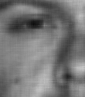
\includegraphics[width = .20 \linewidth]{experimental_evaluation/image_denoising/face_denoising/salt_and_pepper/Figures/yale_06_1_rpca2d_l1_fsim} &
        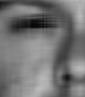
\includegraphics[width = .20 \linewidth]{experimental_evaluation/image_denoising/face_denoising/salt_and_pepper/Figures/yale_06_1_nctrpca_fsim} &
        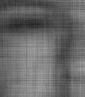
\includegraphics[width = .20 \linewidth]{experimental_evaluation/image_denoising/face_denoising/salt_and_pepper/Figures/yale_06_1_cvpr2016_tnn_fsim}\\
         Noisy & KDRSDL & NC TRPCA & TRPCA '16 \Tstrut\Bstrut \\ \hline
         \textbf{PSNR} & 26.6057 & 22.8502 & 22.566 \Tstrut \\
         \textbf{FSIM} & 0.8956 & 0.8509 & 0.8427
    \end{tabular}
    \caption{Three best results on \textit{Yale} at 60\% noise.}
    \label{tab:top_3_yale_60}
\end{table}
